\documentclass[11pt]{article}

\usepackage{amsmath,amsthm,amssymb}

%%%%% Matrix stretcher
% use it as:
%\begin{pmatrix}[1.5]
% ...
\makeatletter
\renewcommand*\env@matrix[1][\arraystretch]{%
  \edef\arraystretch{#1}%
  \hskip -\arraycolsep
  \let\@ifnextchar\new@ifnextchar
  \array{*\c@MaxMatrixCols c}}
\makeatother
%%%%%%%%%%%%%%%%%%%%%%%%%%

\newcommand\extrafootertext[1]{%
    \bgroup
    \renewcommand\thefootnote{\fnsymbol{footnote}}%
    \renewcommand\thempfootnote{\fnsymbol{mpfootnote}}%
    \footnotetext[0]{#1}%
    \egroup
}


%%%%%%%%%%%%% Colors %%%%%%%%%%%%%
\usepackage[dvipsnames]{xcolor}

\definecolor{C0}{HTML}{1d1d1d}
\definecolor{C1}{HTML}{1e3668}
\definecolor{C2}{HTML}{199d8b}
\definecolor{C3}{HTML}{d52f4c}
\definecolor{C4}{HTML}{5ab2d6}
\definecolor{C5}{HTML}{ffb268}
\definecolor{C6}{HTML}{ff7300} % for commenting - {fire orange}dd571c
\definecolor{C7}{HTML}{777b7e} % for remarks - {steel grey}
\color{C0}
%%%%%%%%%%%%%%%%%%%%%%%%%%%%%%%%



%%%%%%%%%%%%% Fonts %%%%%%%%%%%%% 
%\usepackage{fontspec}
\usepackage[no-math]{fontspec} % for text

\emergencystretch=8pt
\hyphenpenalty=1000 % default 50
\tolerance=800      % default 200
%\righthyphenmin=4
%\lefthyphenmin=4

%%% Text Font: Vollkorn + Math Font: Latin Modern (default) %%%
\setmainfont{Vollkorn}[
UprightFont = Vollkorn-Regular,
ItalicFont =Vollkorn-Italic, 
BoldItalicFont={Vollkorn-BoldItalic},
BoldFont = Vollkorn-Bold,
RawFeature=+lnum,
WordSpace=1.7,
] 

%%% We need this for math font packages other than latin modern %%%
% \usepackage{unicode-math}        % for math

%%% Text Font: Palatino + Math Font: Asana-Math %%%
%\setmainfont{Palatino}[
%BoldFont = Palatino-Bold,
%ItalicFont = Palatino-Italic,
%BoldItalicFont={Palatino-BoldItalic},
%RawFeature=+lnum,
%WordSpace=1.7,
%]
%\setmathfont{asana-math}

%%% Text Font: Arno Pro + Math Font: Minion Pro %%%
%\setmainfont{Arno Pro}[
%UprightFont = *-Regular,
%ItalicFont = Vollkorn-Italic, 
%BoldItalicFont={*-BoldItalic},
%BoldFont = *-Bold,
%RawFeature=+lnum,
%WordSpace=1.7,
%Scale= 1.1
%] 
% Minion Pro is too expensive

%%% Math Fonts %%%
%\setmathfont{Vollkorn}
%\setmathfont{Latin Modern Math}
%\setmathfont{TeX Gyre Pagella Math}
%\setmathfont{TeX Gyre Termes Math}
%\setmathfont{TeX Gyre DejaVu Math}
%\setmathfont[Scale=MatchLowercase]{DejaVu Math TeX Gyre}
%\setmathfont{XITS Math}
%\setmathfont{Libertinus Math}
%\setmathfont[Scale=MatchUppercase]{Asana Math}
%\setmathfont{STIX Two Math}

%\usepackage{kpfonts-otf}
%\setmathfont{KpMath-Regular.otf}[version=regular]
%\setmathfont{KpMath-Bold.otf}[version=bold]
%\setmathfont{KpMath-Semibold.otf}[version=semibold]
%\setmathfont{KpMath-Sans.otf}[version=sans]
%\setmathfont{KpMath-Light.otf}[version=light]


%%% CJK Fonts %%%
\usepackage[scale=.78]{luatexja-fontspec}
\setmainjfont{BabelStone Han}[AutoFakeBold]
%%%%%%%%%%%%%%%%%%%%%%%%%%%%%%%


% This package simplifies the insertion of external multi-page PDF or PS documents.
\usepackage{pdfpages}

% cref
\usepackage{hyperref}
\hypersetup{
    colorlinks=true,
    linkcolor=C4,
    filecolor=magenta,      
    urlcolor=cyan,
    }

\usepackage[nameinlink,noabbrev,capitalize]{cleveref}
% \crefname{ineq}{}{}
% \crefname{equation}{}{}
% \creflabelformat{ineq}{#2{\textup{(1)}}#3}
% \creflabelformat{equation}{#2\textup{(#1)}#3}

%%%%%%%%%%%%% Environments %%%%%%%%%%%%%%%%
%amsthm has three separate predefined styles:	
%
%\theoremstyle{plain} is the default. it sets the text in italic and adds extra space above and below the \newtheorems listed below it in the input. it is recommended for theorems, corollaries, lemmas, propositions, conjectures, criteria, and (possibly; depends on the subject area) algorithms.
%
%\theoremstyle{definition} adds extra space above and below, but sets the text in roman. it is recommended for definitions, conditions, problems, and examples; i've alse seen it used for exercises.
%
%\theoremstyle{remark} is set in roman, with no additional space above or below. it is recommended for remarks, notes, notation, claims, summaries, acknowledgments, cases, and conclusions.

%%%  theorem-like environment %%%
\theoremstyle{plain} % default theorem style
\newtheorem{theorem}{Theorem}[section]
\newtheorem{assumption}[theorem]{Assumption}
\newtheorem{lemma}[theorem]{Lemma}
\newtheorem{corollary}[theorem]{Corollary}
\newtheorem{proposition}[theorem]{Proposition}
\newtheorem{property}[theorem]{Property}

\newtheorem{definition}[theorem]{Definition}

%%% definition-like environment %%%
%\theoremstyle{definition}
\newtheorem{example}[theorem]{Example}
\newtheorem{problem}[theorem]{Problem}


%%% framed package is great %%%
\usepackage{framed}
\newenvironment{solution}
{\color{C2}\normalfont\begin{framed}\begingroup\textbf{Solution:} }
  {\endgroup\end{framed}}

\newenvironment{topic}
{\color{C2}\normalfont\begin{framed}\begingroup }
  {\endgroup\end{framed}}

\newtheoremstyle{remark}% name of the style to be used
  {}% measure of space to leave above the theorem. E.g.: 3pt
  {}% measure of space to leave below the theorem. E.g.: 3pt
  {\color{C3}}% name of font to use in the body of the theorem
  {}% measure of space to indent
  {\color{C3}\bfseries}% name of head font
  {.}% punctuation between head and body
  { }% space after theorem head; " " = normal interword space
  {}
\theoremstyle{remark}
\newtheorem{remarkx}[theorem]{Remark}
\newenvironment{remark}
  {\pushQED{\qed}\renewcommand{\qedsymbol}{$\triangle$}\remarkx}
  {\popQED\endremarkx}
  
\newenvironment{point}
  {\O~~}
  {}

\usepackage{thmtools}
\usepackage{thm-restate}
%%%%%%%%%%%%%%%%%%%%%%%%%%%%%%%%%%%%


% This package is for the long equal sign \xlongequal{}
\usepackage{extarrows}

%%%%%%%%%%%% Algorithms %%%%%%%%%%%%
\usepackage{etoolbox} 
\usepackage{setspace}
\usepackage{algorithm}
\AtBeginEnvironment{algorithmic}{\onehalfspacing}
\usepackage{algorithmicx}
\usepackage[noend]{algpseudocode}

\algrenewcommand\algorithmicindent{2em}
\let\Algorithm\algorithm
\renewcommand\algorithm[1][]{\Algorithm[#1]}%\fontsize{11}{16}\selectfont}

\newenvironment{labelalgorithm}[4][t]{%
\begin{algorithm}[#1]
%\newcommand{\thealgorithmlabel}{#2}
\newcommand{\thealgorithmname}{#3}
%\newcommand{\thealgorithmcap}{#4}
\customlabel{alg:name:#2}{\textproc{#3}}
%\customlabel{alg:cap:#2}{#4}
\caption{#4}\label{alg:#2}
}{\end{algorithm}}

\makeatletter
\newcommand{\customlabel}[2]{%
   \protected@write \@auxout {}{\string \newlabel {#1}{{#2}{\thepage}{#2}{#1}{}} }%
   \hypertarget{#1}{}%
}
\makeatother

%\algdef{SE}[FUNCTION]{Procedure}{EndProcedure}%
%   [2]{\algorithmicclass\ \textproc{#1}\ifthenelse{\equal{#2}{}}{}{$($#2$)$}}%
%   {\algorithmicend\ \algorithmicclass}%

\algnewcommand\algorithmicclass{\textbf{class}}
\algdef{SE}[FUNCTION]{Class}{EndClass}%
   [2]{\algorithmicclass\ \textproc{#1}\ifthenelse{\equal{#2}{}}{}{$($#2$)$}}%
   {\algorithmicend\ \algorithmicclass}%

% Tells algorithmicx not to print an empty line if `noend' is set 
\makeatletter
\ifthenelse{\equal{\ALG@noend}{t}}%
  {\algtext*{EndClass}}
  {}%
\makeatother
%%%%%%%%%%%%%%%%%%%%%%%%%%%%%%%%%%%%


% Page Formatting
\usepackage[
    paper=a3paper,
    inner=22mm,         % Inner margin
    outer=22mm,         % Outer margin
    bindingoffset=0mm, % Binding offset
    top=28mm,           % Top margin
    bottom=22mm,        % Bottom margin
    %showframe,         % show how the type block is set on the page
]{geometry}

\setlength{\parindent}{0em}
\setlength{\parskip}{.7em}


\usepackage{tikz}
\usepackage{graphicx}
\usepackage{subcaption} % for subplots
\usepackage{multicol}   % for multicolumns
\usepackage{wrapfig}    % for inserting figures in multicolumns
\usepackage{enumitem}
\setlist{topsep=0pt}

\usepackage{bm}

\usepackage[font=scriptsize,labelfont=bf]{caption}
\usepackage{listings}
\lstset{basicstyle=\ttfamily,breaklines=true}
% \setlength{\parskip}{1em}
% \setlength{\parindent}{0em}
\usepackage{dsfont}
\newcommand{\bOne}{\mathds{1}}
\newcommand{\PP}{\mathbb{P}}
\newcommand{\EE}{\mathbb{E}}
\newcommand{\VV}{\mathbb{V}}
\newcommand{\CoV}{\operatorname{Co\mathbb{V}}}

% header
\usepackage{fancyhdr}
\pagestyle{fancy}
\fancyhead{}
\fancyhead[L]{\small   \bfseries Notes}
\fancyhead[C]{\small   \bfseries Fall 2023}
\fancyhead[R]{\small   \bfseries Zhou}


\begin{document}

\begin{center}
  \text{\Large{Gaussian Process
    }}

  {\text{Kaiwen Zhou}}
\end{center}
\vspace{2em}

\tableofcontents

%%%%%%%%%%%%%%%%%%%%%%%%%%%%%%
\section*{Readings}
In addition to the lecture notes, the following are required readings:

\begin{itemize}
  \item Chapters 2, 4 Rasmussen (2003)
\end{itemize}

Optional readings:

\begin{itemize}
  \item Sheffield (2007): Gaussian free fields for mathematicians

  \item An excellent intro lecture on Kernel design by Nicolas Durrande can be found in the Sheffield ML summer school on Gaussian Processes

\end{itemize}

%%%%%%%%%%%%%%%%%%%%%%%%%%%%%%
\section{Contextualization: Why do we need the kernel trick?}

\subsection{Feature Map Regression}

\textbf{Supervised Learning and Conditional Expectation:}

The general framework of supervised learning aims to learn a functional
relationshp $y=f(\mathbf{x})$ by optimizing a loss function $L(\mathbf{Y},
  \mathbf{X})=\sum_{i} \ell\left(y_{i}, \mathbf{x}_{i}\right)$ of the training
data $\mathbf{Y},
  \mathbf{X}=\left(y_{i}, \mathbf{x}_{i}\right)$. For quadratic loss, this is the same as
estimating the conditional expectation of $y$ given $\mathbf{x}$ :
$$
  \mathbb{E}[y \mid \mathbf{x}]=\min _{f}|y-f(\mathbf{x})|^{2}
$$
As the above optimization is over all functions, the choice of model amounts to
a choice of parametrizing of a set of functions $\{f(x)\}$, and most ML models fall into the class of
\textbf{additive models} where the function
$f(\mathbf{x})$ can be represented as a sum of base learners:
$$
  f(\mathbf{x})=\sum_{i} f_{i}(\mathbf{x})
$$
For example, OLS, Boosting, Random Forests, most neural nets, Fourier
Transofrms, etc, all fall within this class of additive models.
\vspace*{0.6em}
\hrule

\textbf{Construct the Feature Map Regression:}

Specifically, the feature map regression approach discussed in a previous lecture is an
additive model of the form:
\begin{align}
  f(\mathbf{x}):=\sum_{i}^{N_{F}} \phi_{i}(\mathbf{x}) w_{i}, \quad \text { or } \quad f(\mathbf{X}):=\mathbf{\Phi}(\mathbf{X}) \mathbf{w}
  \label{eq:feature map regression}
\end{align}
where the design matrix for model with $N_{F}$ feature maps and a training set
of $N$ samples $\left(y_{i}, \mathbf{x}_{i}\right)_{i=1}^{N}$ and is defined as:
$$
  \Phi(\mathbf{X}):=\left[\begin{array}{ccc}
      \phi_{1}\left(x_{1}\right) & \cdots & \phi_{N_{F}}\left(x_{1}\right) \\
      \vdots                     &        & \vdots                         \\
      \phi_{1}\left(x_{N}\right) & \cdots & \phi_{N_{F}}\left(x_{N}\right)
    \end{array}\right] \in \mathbb{R}^{N \times N_{F}}
$$
\cref{eq:feature map regression} is a regression model since learners $\phi_{i}$ are
fixed, then so is the design matrix for a given training set ${\mathbf{Y},
      \mathbf{X}}$. Therefore, fitting the model simply amounts to solving for the unknown weights
using the OLS formula:
\begin{align}
  \mathbf{w}^{*} =\min_{\mathbf{w}}\|\mathbf{y}-\mathbf{\Phi}(\mathbf{X}) \mathbf{w}\|^{2}
  =\left(\mathbf{\Phi}(\mathbf{X})^\top \mathbf{\Phi}(\mathbf{X})\right)^{-1} \mathbf{\Phi}(\mathbf{X})^\top \mathbf{y}
  \label{eq:feature map estimator}
\end{align}
Feature map regressions are powerful models because for suitable choices of
$\phi_{i}$, one can approximate most well behaved function.
For example, it turns out that Fourier Series can approximate any
square-integrable function in finite domain $L_{2}$ sense.
Similarly, the Stone-Weierstrass theorem states that the polynomial feature maps
can approximate any continuous function in $L_{1}$ sense (pointwise).
In other words, there exist feature map regression models that are \textbf{universal}. So
why bother with more complex models?
\vspace*{0.6em}
\hrule

\textbf{Curse of Dimensionality of Feature Map Regression:}

Universality comes with a cost. The more flexible a model is, the easier it
would overfit. To avoid such overfitting \cref{eq:feature map estimator} must be regularized, for example,
by adding a shrinkage term:
\begin{align}
  \mathbf{w}^{*}=\left(\mathbf{\Phi}(\mathbf{X})^\top \mathbf{\Phi}(\mathbf{X})+\sigma^{2} \mathbf{I}\right)^{-1} \mathbf{\Phi}(\mathbf{X})^\top \mathbf{y}
  \label{eq:feature map estimator regularized}
\end{align}
However, even if we have regularized, a much bigger issue of \cref{eq:feature
  map estimator regularized} is that it requires the inversion of a $N_{F} \times
  N_{F}$ matrix $\mathbf{A}=\mathbf{\Phi}(\mathbf{X})^\top
  \mathbf{\Phi}(\mathbf{X})+\sigma^{2} \mathbf{I}$. How big is $N_{F}$? We
actually never know! For example, if our feature map model is the Fourier
Transform, this would be equivalent to asking how many Fourier coefficient do we
need to fit a given function to an arbitrary accuracy. In order to be able to
fit any continuous and square integrable function, we would actually need to
include all Fourier components, or equivalently $N_{F} \rightarrow \infty$! As a
result, we would have to invert a $\infty \times \infty$ matrix! That's
impossible, and this is why we need the \textbf{kernel trick} as a work around.

\subsection{The Kernel Trick}

A major simplification occurs if rather than learning the weights $\mathbf{w}$
as in \cref{eq:feature map estimator regularized}, we instead focus on the predictions
given by the linear model. Suppose we train the model on $(\mathbf{y}, \mathbf{X})$
and we wish to predict $\mathbf{y}_{*}=\left(y_{*, j}\right)_{j=1}^{M}$ given
some test inputs $\mathbf{X}_{*}$. By substituting the optimal weights
$\mathbf{w}^{*}$ from \cref{eq:feature map estimator regularized} we have:
\begin{align*}
  \mathbf{y}_{*} & =\mathbf{\Phi}\left(\mathbf{X}_{*}\right) \mathbf{w}^{*}
  =\mathbf{\Phi}\left(\mathbf{X}_{*}\right)\left(\mathbf{\Phi}(\mathbf{X})^\top \mathbf{\Phi}(\mathbf{X})+\sigma^{2} \mathbf{I}\right)^{-1} \mathbf{\Phi}(\mathbf{X})^\top \mathbf{y}                               \\
                 & =\mathbf{\Phi}\left(\mathbf{X}_{*}\right) \sigma^{-2} \mathbf{\Phi}(\mathbf{X})^\top\left(\mathbf{\Phi}(\mathbf{X}) \sigma^{-2} \mathbf{\Phi}(\mathbf{X})^\top+\mathbf{I}\right)^{-1} \mathbf{y} \\
                 & :=K\left(\mathbf{X}_{*}, \mathbf{X}\right)[K(\mathbf{X}, \mathbf{X})+\mathbf{I}]^{-1} \mathbf{y}
\end{align*}

where the kernel matrix (here we only show $K\left(\mathbf{X}_{*}, \mathbf{X}\right)$) is
$$
  K\left(\mathbf{X}_{*}, \mathbf{X}\right) :=\boldsymbol{\Phi}\left(\mathbf{X}_{*}\right) \boldsymbol{\Phi}(\mathbf{X})^\top
  =\left[\begin{array}{ccc}
      K\left(\mathbf{x}_{*, 1}, \mathbf{x}_{1}\right) & \cdots & K\left(\mathbf{x}_{*, 1}, \mathbf{x}_{N}\right) \\
      \vdots                                          &        & \vdots                                          \\
      K\left(\mathbf{x}_{*, M}, \mathbf{x}_{1}\right) & \cdots & K\left(\mathbf{x}_{*, M}, \mathbf{x}_{N}\right)
    \end{array}\right] \in \mathbb{R}^{M \times N}
$$
(the $\sigma^{-2}$ factor was absorbed in the definition of the design
matrix)

The gist here is to realize that even though the design matrix was possibly
infinite dimensional, $\mathbf{\Phi}(\mathbf{X}) \in \mathbb{R}^{N
  \times\left\{N_{F} \rightarrow \infty\right\}}$, this prediction problem only
depends on the kernel matrix $K\left(\mathbf{X}_{*}, \mathbf{X}\right) \in
  \mathbb{R}^{M \times N}$, which is finite dimensional and only depends on the
number of training and test samples, $N, M$. It does not even depend on the
dimensionality $D$ of the features $\mathbf{X} \in \mathbb{R}^{N \times D}$.
Therefore, to do prediction in feature map regression, one does not even need to
fit for the optimal parameters $\mathbf{w}$! The only parameter is the choice of
regularization, $\sigma$.

We will come back shortly to the question of what constitutes a valid Kernel.

\textbf{Bayesian View:}

From the definition in terms of the design matrix, we see that when
evaluated on the train/test dataset, all the kernel matrices
$K\left(\mathbf{X}_{*}, \mathbf{X}_{*}\right), K\left(\mathbf{X}_{*},
  \mathbf{X}\right), K\left(\mathbf{X}, \mathbf{X}_{*}\right)$ and $K(\mathbf{X},
  \mathbf{X})$ are all positive semidefinite. As a result, this suggests that
there is also a probabilistic description of the kernel-trick procedure. Indeed,
the feature map prediction formula can also be derived within a Bayesian
framework as the conditional expectation $\mathbb{E}\left[\mathbf{y}_{*} \mid
    \mathbf{X}_{*}, \mathbf{y}, \mathbf{X}\right]$ of the following probabilistic
model:
\begin{align}
  \begin{bmatrix}
    \mathbf{y} \\
    \mathbf{y}_{*}
  \end{bmatrix} \mid \mathbf{X}, \mathbf{X}_{*}
  \quad \sim \quad
  \mathcal{N}\left(\begin{bmatrix}
                       \boldsymbol{0} \\
                       \boldsymbol{0}
                     \end{bmatrix},
  \begin{bmatrix}
      K(\mathbf{X}, \mathbf{X})+\sigma^{2} \mathbf{I} & K\left(\mathbf{X}, \mathbf{X}_{*}\right)     \\
      K\left(\mathbf{X}_{*}, \mathbf{X}\right)        & K\left(\mathbf{X}_{*}, \mathbf{X}_{*}\right)
    \end{bmatrix}\right)
  \label{eq:kernel as Gaussian Field}
\end{align}

Using the formulas for conditional mean and covariance, then if $\mathbf{X}_{*}
  \neq \mathbf{X}$ we have:
\begin{equation}
  \begin{aligned}
    \mathbb{E}\left[\mathbf{y}_{*} \mid \mathbf{X}_{*}, \mathbf{y}, \mathbf{X}\right]         & =K\left(\mathbf{X}_{*}, \mathbf{X}\right)\left[K(\mathbf{X}, \mathbf{X})+\sigma^{2} \mathbf{I}\right]^{-1} \mathbf{y}                                                                             \\
    \operatorname{Cov}\left[\mathbf{y}_{*} \mid \mathbf{X}_{*}, \mathbf{y}, \mathbf{X}\right] & =K\left(\mathbf{X}_{*}, \mathbf{X}_{*}\right) -K\left(\mathbf{X}_{*}, \mathbf{X}\right)\left[K(\mathbf{X}, \mathbf{X})+\sigma^{2} \mathbf{I}\right]^{-1} K\left(\mathbf{X}, \mathbf{X}_{*}\right)
  \end{aligned}
  \label{eq: posterior predictive distribution}
\end{equation}

If on the other hand $\mathbf{X}_{*}=\mathbf{X}$ and $\sigma=0$, then
$\mathbb{E}\left[\mathbf{y}_{*} \mid \mathbf{X}, \mathbf{y},
    \mathbf{X}\right]=\mathbf{y}$ and $\operatorname{Cov}\left[\mathbf{y}_{*} \mid
    \mathbf{X}, \mathbf{y}, \mathbf{X}\right]=0$. In this case, there is no uncertainty of the
posterior predictions as they are assumed to equal the prior observations,
$\mathbb{E}\left[\mathbf{y}_{*} \mid \mathbf{X}, \mathbf{y},
    \mathbf{X}\right]=y$.

Note that the posterior conditional expectation formula in the first equation
above is the same as the prediction formula for feature map regression after
the kernel trick is applied.

%%%%%%%%%%%%%%%%%%%%%%%%%%%%%%
\section{Topic: Gaussian Process}

Gaussian Fields are a multi-dimensional generalization of Gaussian Processes.
However in the ML community the two names are used interchangeably. As a
reminder, a Gaussian Process is a familiar concept in stochastic theory:

\begin{definition}\textbf{(Gaussian Fields)}
  A continuous real (stochastic) function $Y_{\mathrm{x}}:=Y(\mathrm{x}):
    \mathbb{R}^{D} \rightarrow R$ is a Gaussian Field if and only if for any set of
  points $\left(x_{i}\right)_{i=1}^{k}$, the $k-$ dimensional variable
  $$
    \mathbf{Y}_{\mathbf{x}_{1}, \ldots, \mathbf{x}_{k}}:=\left(Y_{\mathbf{x}_{1}}, \ldots, Y_{\mathbf{x}_{k}}\right)
  $$
  is a multivariate Gaussian random variable. Equivalently, every linear
  combination $\mathbf{w} \cdot \mathbf{Y}_{\mathbf{x}_{1}, \ldots,
    \mathbf{x}_{k}}$ has a univariate Gaussian distribution.
\end{definition}

\begin{definition}\textbf{(Gaussian Process)}
  A time continuous stochastic process $\left\{X_{t}, t \in T\right\}$ is a
  Gaussian Process if and only for every set of indices
  $\left(t_{i}\right)_{k=1}^{k}$ in the index set $T$ the $k$-dimensional variable
  $$
    \mathbf{X}_{t_{1}, \ldots, t_{k}}:=\left(X_{t_{1}}, \ldots, X_{t_{k}}\right)
  $$
  is a multivariate Gaussian random variable. Equivalently, every linear
  combination $\mathbf{w} \cdot \mathbf{X}_{t_{1}, \ldots, t_{k}}$ has a
  univariate Gaussian distribution.
\end{definition}

\begin{figure}[!htp]
  \centering
  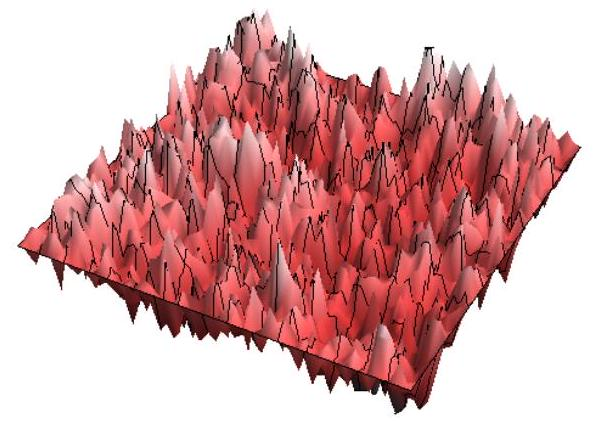
\includegraphics[width=0.3\textwidth]{images/2023_11_26_5b299dbd302e8f129737g-22}
  \caption{A 2D Gaussian Field.}
  \label{fig:2D Gaussian Field}
\end{figure}

%%%%%%%%%%%%%%%%%%%%%%%%%%%%%%%%%%%%
\section{Topic:  Kernel Design}

What is a Kernel? It is clear that \cref{eq:kernel as Gaussian Field} is a Gaussian Field due to the fact that
the kernel matrices entering into the equation are all positive semidefinite.
This motivates the following

\begin{definition}
  \textbf{(Kernel)} A kernel is a continuous function $K: \mathbb{R}^{D} \times \mathbb{R}^{D}
    \rightarrow \mathbb{R}$ with the following properties (\href{https://en.wikipedia.org/wiki/Mercer%27s_theorem}{Mercer Conditions}):
  \begin{enumerate}
    \item $K$ is symmetric: $K(\mathbf{x}, \mathbf{y})=K(\mathbf{y}, \mathbf{x})$
    \item $K$ is positive semidefinite, i.e. for any finite set of points
          $\left(x_{i}\right)_{i=1}^{n}$ we have
          $$
            \sum_{i=1}^{n} \sum_{j=1}^{n} K\left(\mathbf{x}_{i}, \mathbf{x}_{j}\right) c_{i} c_{j} \geq 0
          $$
          for all choices of real numbers $\left(c_{i}\right)_{i=1}^{n}$.
  \end{enumerate}
\end{definition}

\subsection{Valid Kernels}
Which Symmetric Functions are Valid Kernels? Given any symmetric real function
$K(\mathbf{x}, \mathbf{y})$ it turns out it is not generally easy to show that
the function defines a valid Kernel. We will elaborate on this later. However,
it turns out that there are several easy ways to generate new kernels from old
as follows.

\begin{proposition}\textbf{(Valid Kernel Properties)}\hfill
  \begin{enumerate}[label=(\alph*)]
    \item \textbf{Product of Valid Kernels is a Valid Kernel:}
          Given two valid kernels $K_{1}$ and $K_{2}$, the product $K=K_{1} K_{2}$ is a
          valid kernel.
    \item \textbf{Sum of Valid Kernels is a Valid Kernel:}
          Given two valid kernels $K_{1}$ and $K_{2}$, the sum $K=K_{1}+K_{2}$ is a valid kernel.
    \item \textbf{Corollary - Mixture of Valid Kernels is a Valid Kernel:}
          Given two valid kernels $K_{1}$ and $K_{2}$ and $a \geq 0, b \geq 0$, then $K=aK_{1}+b K_{2}$ is a valid kernel for $a, b \geq 0$. One often also assumes
          $a+b=1$.
    \item \textbf{Composition Kernel:}
          If $K_{1}: \mathbb{R}^{D \times D} \rightarrow \mathbb{R}$ is a valid Kernel and
          $\mathbf{f}: \mathbb{R}^{N} \rightarrow \mathbb{R}^{D}$ is any vector function,
          then $K(\mathbf{x}, \mathbf{y}):=K_{1}(\mathbf{f}(\mathbf{x}),
            \mathbf{f}(\mathbf{y}))$ is also a valid Kernel.
    \item \textbf{Corollary - Periodic Kernel from a given kernel}
          If $\mathrm{f}$ is a periodic function, then $K$ above would be a periodic
          Kernel generating paths with the same periodicity as $\mathbf{f}$.
    \item \textbf{Tensor Product/Sum Kernel:}
          Suppose $K_{1}: \mathbb{R}^{D_{1} \times D_{1}} \rightarrow \mathbb{R}$ and
          $K_{2}: \mathbb{R}^{D_{2} \times D_{2}} \rightarrow \mathbb{R}$ are valid
          kernels. Suppose also $\mathbf{z}:=(\mathbf{x} ; \mathbf{y}) \in
            \mathbb{R}^{D_{1}+D_{2}}$ where $\mathbf{x} \in \mathbb{R}_{1}^{D}$ and
          $\mathbf{y} \in \mathbb{R}_{2}^{D}$. Then both $K(\mathbf{z},
            \mathbf{z})=K_{1}(\mathbf{x}, \mathbf{x})+K_{2}(\mathbf{y}, \mathbf{y})$ and
          $K(\mathbf{z}, \mathbf{z})=K_{1}(\mathbf{x}, \mathbf{x}) K_{2}(\mathbf{y},
            \mathbf{y})$ are valid kernels.
  \end{enumerate}
\end{proposition}

\begin{proposition}\textbf{(Linear (Dot Product) Kernel)}
  $K(\mathbf{x}, \mathbf{y})=\mathbf{x}^{T} \mathbf{y}$ is a valid kernel for any
  $\mathbf{x}, \mathbf{y} \in \mathbb{R}^{D}$ (why?).
\end{proposition}

\begin{figure}[!htp]
  \centering
  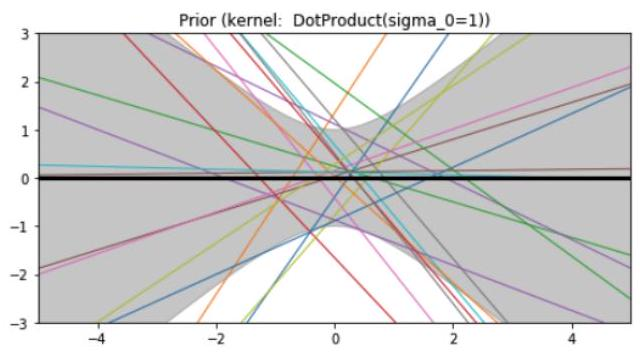
\includegraphics[width=0.4\textwidth]{images/2023_11_26_5b299dbd302e8f129737g-35}
  \caption{Prior paths from the Linear (Dot Product) Kernel mixed with a Constant Variance Kernel, $K(x, y)=\sigma^{2}+x y$.}
  \label{fig:Linear (Dot Product) Kernel}
\end{figure}

Even though technically $K(\mathbf{x}, \mathbf{y})$ is a quadratic function,
this is called a linear Kernel, because the posterior expectation and covariance
formulas \cref{eq: posterior predictive distribution} for this Kernel would correspond to those of linear regression.

\begin{proposition}\textbf{(Feature Map Kernel)}
  $K(\mathbf{x}, \mathbf{y})=\phi(\mathbf{x}) \phi(\mathbf{y})$ is a valid
  kernel for any $\phi(\mathbf{x}): \mathbb{R}^{D} \rightarrow R$.

  One way to show that this is a valid kernel directly from the
  definition and (66). Alternatively, the scalar Linear Kernel $K(t, s)=t s$ is
  seen as a valid Kernel for scalar $t, s \in R$. The result then follows by
  realizing that the Feature Map kernel is a Composition Kernel of the scalar
  Linear Kernel.
\end{proposition}


\subsection{Feature Map Kernel: Connection to Stochastic Processes/Fields}
\textbf{1-D Features: The Kernel of a Stochastic Process}

For a one-dimensional square-intergrable zero-mean continuous process $Y_{t}$
over a probability space $(\Omega, \mathcal{F}, \mathbb{P})$ indexed over the closed
interval $[a, b]$ the following function $K_{Y}(s, t)$ is a valid Kernel (show
this!):
$$
  K_{Y Y}(s, t)=\mathbb{E}\left[Y_{s} Y_{t}\right]
$$

In time-series analysis the above Kernel is known as the level-Autocovariance
Function (ACF).

Square-integrability is needed to ensure that the total variance $V=\int_{a}^{b}
  \mathbb{E}\left[Y_{t}^{2}\right] d t=\int_{a}^{b} K_{Y Y}(t, t) d t$ of the
process is finite.


Corollary

Given a square-integrable $\Pi_{t}=\int_{a}^{t} \Delta_{s} Y_{s} d s$ the
following is a valid Kernel:

$$
  K_{\Pi \Pi}\left(t, t^\top\right)=\mathbb{E}\left[\Pi_{t} \Pi_{t}^\top\right]=\mathbb{E}\left[\int_{a}^{t} \Delta_{s} Y_{s} d s \int_{a}^{t^\top} \Delta_{s}^\top Y_{s}^\top d s^\top\right]
$$

The above theorem and corollary allow us to construct kernels corresponding to a
any specified stochastic process.

\begin{example}
  \textbf{(White-Noise Kernel)} The Kernel of $d W_{t} \sim N(0, d t)$ is
  $$
    K_{\text {noise }}(s, t)=d t \bOne_{s, t}
    \quad \text{ where } \quad
    \bOne_{s, t}=
    \begin{cases}
      1 \text{ if } s=t \\
      0 \text{ if } s\neq t
    \end{cases}
  $$
\end{example}

\begin{example}
  \textbf{(Brownian Kernel)} The Kernel of $X_{t}=\int_{0}^{t} d W_{s}$ is:
  $$
    K_{B M}(s, t)=\min (t, s) .
  $$
  Note that for time-varying vol process $d X_{t}=\sigma(t) d W_{t}$ the Kernel is
  $K\left(t, t^\top\right)=\min \left(\int_{0}^{t} \sigma^{2}(s) d s,
    \int_{0}^{t^\top} \sigma^{2}\left(s^\top\right) d s^\top\right)=\min \left(Q V
    S(t), Q V S\left(t^\top\right)\right)$ where $Q V
    S(t)=\mathbb{E}\left[X_{t}^{2}\right]=\mathbb{E}\left[\int_{0}^{t} d
      X_{s}^{2}\right]=\int_{0}^{t} \sigma^{2}(s) d s$ is the quadratic variance swap
  of $X_{t}$.
\end{example}

\begin{example}
  \textbf{(Bachelier Local-Vol Kernel)} The Kernel of the Bachelier Local-Vol process $d X_{t}=\sigma^{2}\left(X_{t},
    t\right) d W_{t}$ is:
  $$
    K_{L V}(s, t)=\mathbb{E}\left[X_{s} X_{t}\right]=\min \left(Q V S(t), Q V S\left(t^\top\right)\right)
  $$
  where $Q V S(t)=\mathbb{E}\left[X_{t}^{2}\right]=\mathbb{E}\left[\int_{0}^{t} d
      X_{s}^{2}\right]=\mathbb{E}\left[\int_{0}^{t} \sigma^{2}\left(X_{s}, s\right) d
      s\right]$.
\end{example}

\begin{example}
  \textbf{(Ornstein-Uhlenbeck Kernel)} For sufficiently large $t, s \gg a=0$, the Kernel of the OU process $d
    x_{t}=-\alpha d t+\sigma d W_{t}$ is:
  \begin{align}
    K_{O U}(s, t)=\frac{\sigma^{2}}{2 \alpha} e^{-\alpha|t-s|}
    \label{eq: OU kernel}
  \end{align}
\end{example}

\textbf{N-D Features: The Kernel of a Stochastic Process}

For a $N$-dimensional square-intergrable zero-mean continuous field
$Y_{\mathbf{x}}$ over a probability space $(\Omega, \mathcal{F}, \mathbb{P})$ indexed over
some compact space $C$ (for example $C=[0,1]^{N} \subset \mathbb{R}^{N}$ ), then
the following function $K_{Y Y}\left(\mathbf{x}, \mathbf{x}^{\prime}\right)$ is a
valid Kernel:
$$
  K_{Y Y}\left(\mathbf{x}, \mathbf{x}^{\prime}\right)=\mathbb{E}\left[Y_{\mathbf{x}} Y_{\mathbf{x}^{\prime}}\right]
$$
This would be a higher-dimensional generalization of the ACF.
Square-integrability is needed again to ensure that the total variance
$V=\int_{C} \mathbb{E}\left[Y_{\mathbf{x}}^{2}\right] d \mathbf{x}=\int_{C} K_{Y
      Y}(\mathbf{x}, \mathbf{x}) d \mathbf{x}$ of the process is finite.

\begin{example}
  \textbf{(N-D Brownian Motion Kernel)} Suppose $\mathbf{Y}_{t} \in R^{N}$ be
  the level of $N$-dimensional correlated Brownian motion over a finite $t$ -
  domain (to ensure square-integrability):
  $$
    \mathbf{Y}_{t}=\int_{0}^{t} d \mathbf{W}_{s}, \quad \mathbb{E}\left[d W_{t, i} d W_{t, i}\right]=C_{i j} d t
  $$
  Define $x:=(t, i), \quad t \in[0,1], i \in 1, \ldots, N$ as well as the r.v.
  $Z_{\mathrm{x}}:=Y_{t, i}$ we have:
  $$
    K_{N d B M}\left(\mathbf{x}, \mathbf{x}^{\prime}\right)=\mathbb{E}\left[Z_{\mathbf{x}}, Z_{\mathbf{x}^{\prime}}\right]=\mathbb{E}\left[Y_{t, i} Y_{t^{\prime}, i^{\prime}}\right]=\min \left(t, t^{\prime}\right) C_{i i^{\prime}}
  $$
\end{example}

\subsection{Application: Futures Curve Modeling}
Simply replace the asset index $i$, with $\tau=T-t$ of a continuously rolled
constant time-to-maturity strategy. As there is a continuum of $\tau$ we have
$\mathbf{Y}_{t}=\left(Y_{t, \tau}\right)_{\tau} \in
  \mathbb{R}_{+}^{\mathbb{R}}$. Ignoring the carry drift, we are then modeling:

$$
  \mathbf{Y}_{t}=\int_{0}^{t} d \mathbf{W}_{s}, \quad \mathbb{E}\left[d W_{t, \tau} d W_{t, \tau^{\prime}}\right]=C\left(\tau, \tau^{\prime}\right) d t
$$

Define $x:=(t, \tau), \quad t \in[0,1], \tau \in \mathbb{R}_{+}$as well as the
r.v.

$Z_{\mathrm{x}}:=Y_{t, \tau}$ we have:

$$
  K\left(\mathbf{x}, \mathbf{x}^{\prime}\right)=\mathbb{E}\left[Z_{\mathbf{x}}, Z_{\mathbf{x}^{\prime}}\right]=\mathbb{E}\left[Y_{t, \tau} Y_{t^{\prime}, \tau^{\prime}}\right]=\min \left(t, t^{\prime}\right) C\left(\tau, \tau^{\prime}\right)
$$

The same construction generalizes to higher dimensional features instead of
$\tau$ where in a similar manner the Kernel would be the tensor product of a
time component $\min \left(t, t^{\prime}\right)$ and a spatial/feature component.

\subsection{Stationary Kernels}
In time-series analysis, stationary processes processes are such that their ACF
is time-homogeneous. A generalization in $N-D$ is the following:

\begin{definition}\textbf{(Stationary Kernel)}
  A Kernel is stationary if $$K(\mathbf{x}, \mathbf{y})=K(\mathbf{x}-\mathbf{y})$$
\end{definition}

\begin{corollary}
  Due to the fact that a Kernel is a symmetric function, if a Kernel is stationary then
  $$K(\mathbf{x},
    \mathbf{y})=K(\boldsymbol{\tau})=K(-\boldsymbol{\tau})=K(|\boldsymbol{\tau}|),
    \quad \boldsymbol{\tau}:=\mathbf{x}-\mathbf{y}$$
\end{corollary}

\begin{theorem}
  \textbf{(Bochner's Theorem)} A function $K: \mathbb{R}^{D} \rightarrow \mathbb{R}$ is a stationary kernel,
  i.e. the $A C F$ of a stationary square-integrable field, if and only if it can
  be represented as:
  $$
    K(\boldsymbol{\tau})=\int_{R^{D}} e^{2 \pi i \boldsymbol{\omega} \cdot \boldsymbol{\tau}} d \mu(\boldsymbol{\omega})
  $$
  where $\mu$ is a unique positive measure.
\end{theorem}

For the case of $\tau \in R$, Bochner's Theorem is also known as the following:
\begin{theorem}
  \textbf{(Wiener-Khinchine Theorem)} For every stationary continuous-time square-integrable stochastic process
  $x_{t}$ there exists a monotone function $F(f)$ such that the
  level-autocovariance of the process $K_{X X}(\tau)=\mathbb{E}\left[X_{t}
      X_{t-\tau}\right]$ can be written as:
  $$
    K_{X X}(\tau)=\int_{-\infty}^{\infty} e^{2 \pi i f \tau} d F(f)
  $$
\end{theorem}

In the $N$-D case we write $d \mu(\omega)=S(\omega) d \omega$, then $S(\omega)$
is called the spectral density of the Kernel/process. Essentially this is the
Fourier transform of the Kernel:

$$
  S(\boldsymbol{\omega})=\int e^{-2 \pi i \boldsymbol{\omega} \cdot \boldsymbol{\tau}} K(\boldsymbol{\tau}) d \boldsymbol{\tau}
$$

Note that $K(\mathbf{0})=\int S(\boldsymbol{\omega}) d \boldsymbol{\omega}$ must
be finite for square-integrable field (why?), which is why without loss of
generality the process

can be rescaled so that $\int d \mu(\boldsymbol{\omega})=\int
  S(\boldsymbol{\omega}) d \boldsymbol{\omega}=1$.

Square-integrability is therefore requred in order to ensure that $d \mu$ is a
proper measure.

\textbf{Stationary Kernels: Intuition}

Because the Kernel (or variance-covariance) $K(\mathbf{x}, \mathbf{y})$ only
depends on the distance $|\mathbf{x}-\mathbf{y}|$ between $\mathbf{x}$ and
$\mathbf{y}$, but not on the actual positions $\mathbf{x}, \mathbf{y}$, the
local variability of the prior paths/surfaces generated by stationary Kernels is
the same throughout the entire domain. Non-stationary kernels, on the other
hand, generate spatially varying local variance/covariance of the prior
paths/surfaces.

For example, the linear kernel is not stationary, as is clearly also visible in
\cref{fig:Linear (Dot Product) Kernel}. An example of a stationary Kernel is that of the OU process (11) whose prior
paths can be seen below:

\begin{figure}[!htp]
  \centering
  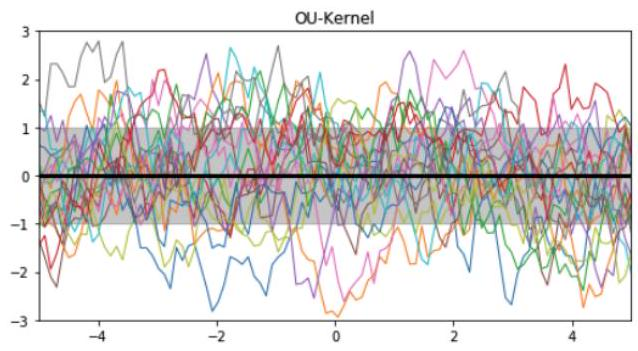
\includegraphics[width=0.3\textwidth]{images/2023_11_26_5b299dbd302e8f129737g-55}
  \caption{Prior paths from OU Kernel (or $\nu=1 / 2$ Matern Kernel with scale
    parameter $\ell), K(x, y)=\exp (-\tau / \ell)$.}
  \label{fig:stationary Matern kernel}
\end{figure}

\begin{example} \textbf{(Examples of Stationary Kernels)}
  \begin{itemize}
    \item OU Kernel in \cref{eq: OU kernel}.

    \item RBF Kernel: $K_{R B F}\left(\mathrm{x}, \mathrm{x}^\top\right)=K_{R B
            F}(\tau)=\exp \left(-\tau^{2} / 2 \ell^{2}\right)$, where
          $\tau=\sqrt{\tau}=\sqrt{\left|\mathrm{x}-\mathrm{x}^{prime}\right|}$ where
          $\ell>0$ is the scale hyperparameter of the Kernel. Why is this a valid
          Kernel?

    \item Matern Kernel: $K_{\text {Matern
                }}(\tau)=\frac{2^{1-\nu}}{\Gamma(\nu)}\left(\frac{\sqrt{2 \nu}
              \tau}{\ell}\right)^{\nu} K_{\nu}\left(\frac{\sqrt{2 \nu} \tau}{\ell}\right)$
          where $\nu, \ell>0$ are the hyperparameters of the Kernel. It turns out that
          as $\nu \rightarrow \infty$ the Matern Kernel becomes the RBF Kernel $K_{\text
                {Matern }} \rightarrow \exp \left(-\tau^{2} / 2 \ell^{2}\right)$ while when
          $\nu=1 / 2$ it becomes the OU Kernel $\left.K_{\text {Matern }}\right|_{\nu=1
            / 2}=\exp (-\tau / \ell)$

    \item $\gamma$-exponential Kernel: $K_{\gamma-\operatorname{Exp}}(\tau)=\exp
            \left(-(\tau / \ell)^{\gamma}\right), 0<\gamma \leq 2$

    \item Rational-Quadratic Kernel: $K_{R Q}(\tau)=\left(1+\frac{\tau^{2}}{2
              \alpha \ell^{2}}\right)^{-\alpha}$

    \item Anisotropic stationary Kernels: Simply set
          $\tau^{2}=\left(\mathrm{x}-\mathrm{x}^{prime}\right)^\top
            \mathbf{S}^{-1}\left(\mathrm{x}-\mathrm{x}^{prime}\right)$ where $\mathbf{S}$ is
          a positive-definite matrix.

    \item Anisotropic factor models: In the above we simply specify the $D \times
            D$ matrix $\mathrm{S}$ by its dimensionally reduced factor structure
          $\mathbf{S}=\mathbf{V} \mathbf{V}^\top+\mathbf{R}$ where $\mathbf{V}$ is a $D
            \times k$ matrix specifying the loadings of the $k$ factors and $\mathbf{R}$
          is a diagonal positive definite matrix specifying the idiosyncratic variances
          of each of the coordinates of $\mathbf{x}$
  \end{itemize}
\end{example}


\section{Bayesian Learning With GPs}
\textbf{Generating From The Prior}

Generating from the prior amounts to choosing a set of test grid points
$\mathbf{X}_{*}=\left(\mathbf{x}_{*, i}\right)_{i=1}^{M}$ and generating
different realizations of $\mathbf{y}_{*}=\left(y_{*, i}\right)_{i=1}^{M}$ by
drawing from the following multivariate Gaussian (prior) distribution 
$$
  \mathbf{y}_{*} \mid \mathbf{X}_{*} \sim N\left(0, K\left(\mathbf{X}_{*}, \mathbf{X}_{*}\right)\right)
$$

\begin{figure}[!htp]
  \centering
  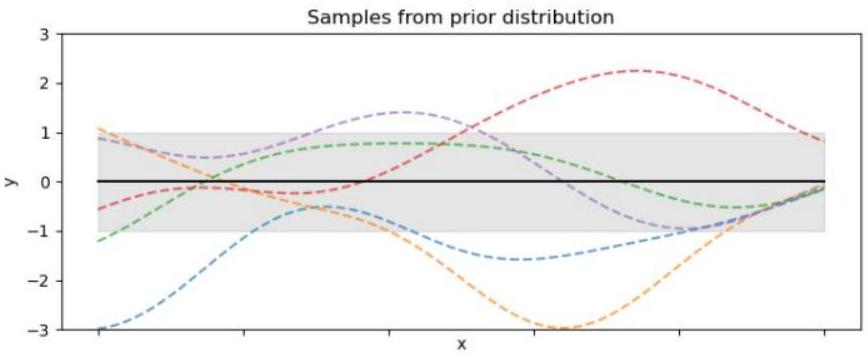
\includegraphics[width=.6\textwidth]{images/2023_11_26_5b299dbd302e8f129737g-23}
      \caption{Sample paths from the prior of the RBF Kernel $K\left(x_{1},
      x_{2}\right)=\exp \left(-\left|x_{1}-x_{2}\right|^{2} /
      \sigma^{2}\right)$}
      \label{fig:RBF Kernel prior}
\end{figure}

\textbf{Training and Generating From The Posterior}

Generating from the posterior amounts to choosing a set of test grid points
$\mathbf{X}_{*}=\left(\mathbf{x}_{*, i}\right)_{i=1}^{M}$ and generating
different realizations of $\mathbf{y}_{*}=\left(y_{*, i}\right)_{i=1}^{M}$ by
drawing from the posterior multivariate Gaussian distribution in (24)
$$
  \mathbf{y}_{*} \mid \mathbf{X}_{*}, \mathbf{y}, \mathbf{X} \sim N\left(\mathbb{E}\left[\mathbf{y}_{*} \mid \mathbf{X}_{*}, \mathbf{y}, \mathbf{X}\right], \operatorname{Cov}\left[\mathbf{y}_{*} \mid \mathbf{X}_{*}, \mathbf{y}, \mathbf{X}\right]\right)
$$
where the conditional mean and covariance are as in (16).

\begin{figure}[!htp]
  \centering
  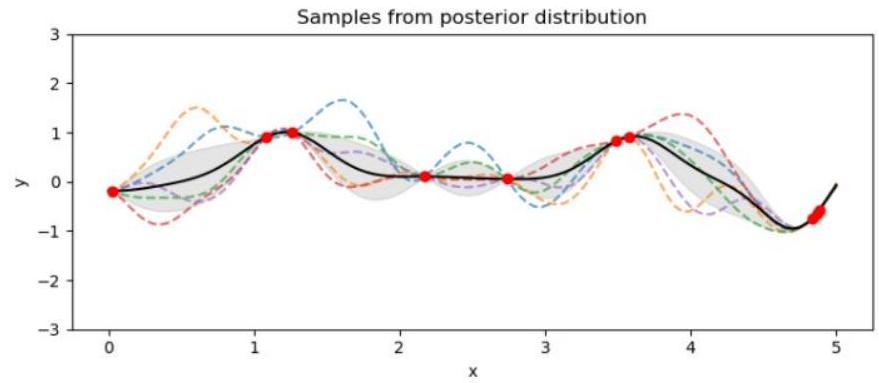
\includegraphics[width=0.6\textwidth]{images/2023_11_26_5b299dbd302e8f129737g-25}
  \caption{Sample paths from the posterior of the RBF Kernel $K\left(x_{1}, x_{2}\right)=\exp \left(-\left|x_{1}-x_{2}\right|^{2} /
  \sigma^{2}\right)$ based on a training set of only 9 samples.}
  \label{fig:RBF Kernel posterior}
\end{figure}

\section{Model Selection and Hyperparameter Optimization}

\section*{What is GPR Model Selection? I}
As we noted earlier, the training of a Gaussian Process (16) for a fixed Kernel
does not involve fitting any parameters. In other words, we have solved the
$L_{2}$ optimization problem for the predictions $\mathbf{y}_{*}$ conditional on
$\mathbf{X}_{*}$ and training data $\mathbf{y}, \mathbf{X}$ in a single
optimization step.

However, in many cases the Kernel itself may depend, generally in a non-linear
fashion, on a set of hyperparameters $\theta$, $K\left(\mathrm{x},
\mathrm{x}^{\prime}\right)=K\left(\mathrm{x}, \mathrm{x}^{\prime} ;
\theta\right)$. For example, the $\ell$ parameter in the RBF Kernel is a
hyperparameter.

\section*{What is GPR Model Selection? II}
If $\ell$ is too small, the bandwidth of the Kernel may be too narrow and the
model overfits:

\begin{center}
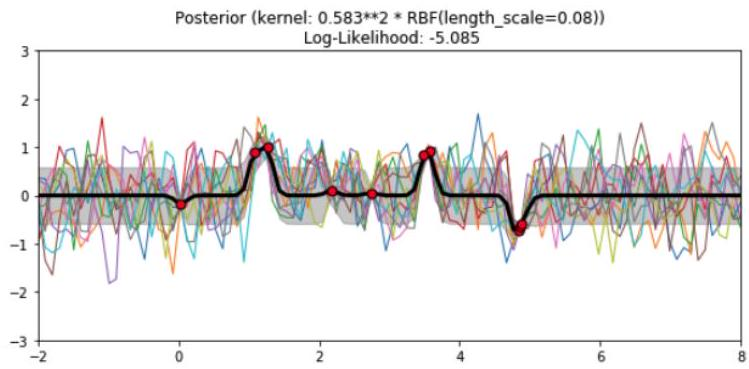
\includegraphics[width=\textwidth]{images/2023_11_26_5b299dbd302e8f129737g-60}
\end{center}

Figure 6: An RBF fit with narrow bandwidth.

\section*{What is GPR Model Selection? III}
If $\ell$ is too large, the bandwidth of the Kernel may be too wide and the
model underfits:

\begin{center}
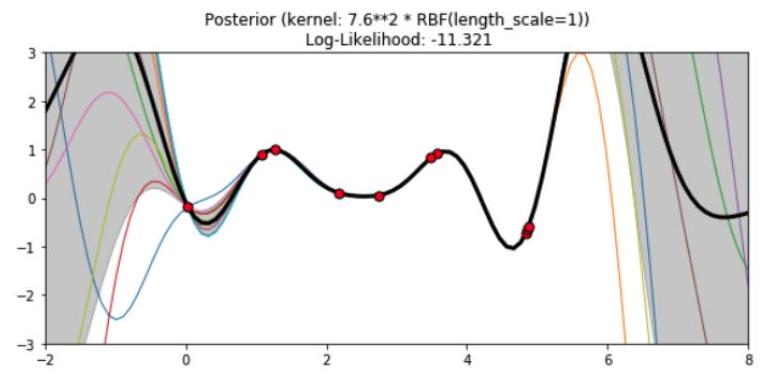
\includegraphics[width=\textwidth]{images/2023_11_26_5b299dbd302e8f129737g-61}
\end{center}

Figure 7: An RBF fit with wide bandwidth.

\section*{What is GPR Model Selection? IV}
The optimal $\ell$ balances the bias-variance tradeoff.

\begin{center}
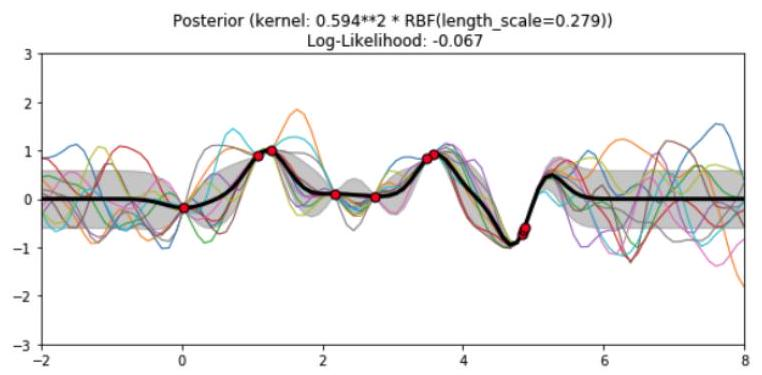
\includegraphics[width=\textwidth]{images/2023_11_26_5b299dbd302e8f129737g-62}
\end{center}

Figure 8: The optimal bandwidth RBF fit.

One way to find $\theta_{\text {opt }}$ would be through grid search and
crossvalidation. However in bayesian modelling there is typically insufficient
training data to adopt this approach. What are the alternatives?

\section*{Optimizing the Likelihood of the Data I}
Within the Bayesian framework, hyperparameter optimization amounts to optimizing
the likelihood of the data as a function of the hyperparameters:

$$
\begin{aligned}
L(\theta \mid \mathbf{y}, \mathbf{X}) & =\log p(\mathbf{y} \mid \mathbf{X} ; \boldsymbol{\theta}) \\
& =-\frac{1}{2} \mathbf{y}^{\prime}\left(K(\mathbf{X}, \mathbf{X} ; \boldsymbol{\theta})+\sigma^{2} \mathbf{I}\right)^{-1} \mathbf{y} \\
& -\frac{1}{2} \log \left|\left(K(\mathbf{X}, \mathbf{X} ; \boldsymbol{\theta})+\sigma^{2} \mathbf{I}\right)\right|-\frac{n}{2} \log 2 \pi
\end{aligned}
$$

\section*{Optimizing the Likelihood of the Data II}
In general (63) is non-trivial both because of the non-linear dependence in
$\theta$ and because of the fact that at gradient optimization step the inverse
of $K(\mathbf{X}, \mathbf{X} ; \boldsymbol{\theta})+\sigma^{2} \mathbf{I}$ would
have to be computed.

Fortunately, in many problems one does not require many hyperparameters to
optimize over. Quite often, using a simple Kernel such as the RBF one suffices
in getting good results. However, hyperparameter optimization is in fact one of
the biggest bottlenecks of the GPR approach, especially in the limit of large
amounts of data. On the other hand, Bayesian approach is precisely most useful
in the oposite limit of small amounts of data which is especially relevant to
finance.

%%%%%%%%%%%%%%%%%%%%%%%%%%%%%%%%%%%%%%%%%%%%%%
\section{Links to SVD/PCA: Mercer's Theorem, Karhunen-Loève Expansion And Their Generalizations}
\subsection{Mercer's Theorem}
In a previous section we found that a sufficient condition for a Kernel to be
valid is to express it as a covariance function, or alternatively a quadratic
outer product of a set of feature maps, $K\left(\mathrm{x},
\mathrm{x}^{\prime}\right)=\boldsymbol{\Phi}(\mathrm{x})
\boldsymbol{\Phi}\left(\mathrm{x}^{\prime}\right)^{\prime}=\sum_{\alpha}
\phi_{\alpha}(\mathrm{x}) \phi_{\alpha}\left(\mathrm{x}^{\prime}\right)$ in
which case the second Mercer condition follows directly.

Under what condition does the reverse hold, i.e. that we can decompose a Kernel
as an outer product of feature maps? The following theorem shows that the Mercer

\section*{Mercer's Theorem II}
Theorem (Merce, '1909)

Every valid Kernel in $1-D$, i.e. a symmetric function

$K(s, t), s, t \in[a, b]$ satisfying the Mercer condition (66), can be expressed
as:

$$
K(s, t)=\sum_{i=1}^{\infty} \lambda_{i} e_{i}(s) e_{i}(t)
$$

where $\left\{\lambda_{i} \geq 0, e_{i}(t)\right\}_{i=1}^{\infty}$ are the
solutions of the following Friedholm Integral Eigenvalue equation:

$$
\int_{a}^{b} K_{Y}(s, t) e_{k}(s) d s=\lambda_{k} e_{k}(t)
$$

and $\left\{e_{i}(t)\right\}_{i=1}^{\infty}$ are orthonormal wrt the Hilbert
norm

$\left\langle e_{i}, e_{j}\right\rangle_{\mathcal{H}}:=\int_{a}^{b} e_{i}(t)
e_{j}(t) d t=\delta_{i j}$.

\section*{Mercer's Theorem III}
The feature maps $e_{i}(t)$ are the functional analogue of PCA factors of the
Kernel. Indeed, they are orthonormal wrt the Hilbert norm

$\langle,\rangle_{\mathcal{H}}$ and so they form a complete basis of functions
which are linear superspositions of the factors. What can we say about such
functions?

\section*{The Hilbert Space of the Kernel I}
Consider the functions generated by this Mercer orthonormal basis associated
with a given Kernel:

$$
f(t)=\sum_{i=0}^{\infty} \alpha_{i} e_{i}(t)
$$

It is easy to check that these functions form a real vector space embodied with
an inner product $\langle\rangle=,\langle,\rangle_{\mathcal{H}}$. In other words
these functions form a Hilbert Space $H$.

\section*{The Hilbert Space of the Kernel II}
What type of functions are in $H$ ?

For example, if each of the basis functions
$\left\{e_{i}(t)\right\}_{i=1}^{\infty}$ were differentiable it is clear that if
one were to consider functions in (47) generated by finitely many of the basis
vectors, then the result would be differentiable as well.

As differentiable functions have zero quadratic variation, so would this imply
that the Hilbert space $H$ only consists of deterministic functions?

\section*{The Hilbert Space of the Kernel III}
It turns out the answer is no precisely because the expansions in

(47) constitue of countably infnite series of superpositions of
$\left\{e_{i}(t)\right\}$.

In fact, if the Kernel is a covariance of a given square-integrable stochastic
process, then it turns out that there exists a sequence of functions in
$\mathrm{H}$ which converges in $L_{2}$-sense to any given path of the process.

\section*{Karhunen-Loève (KL) Expansion I}
Suppose $K(t, s)=\mathbb{E}\left[Y_{t} Y_{s}\right]$ for a zero-mean
square-integrable process over a probability space $(\Omega, F, \mathbf{P})$
indexed over the closed interval $[a, b]$. Then $K(t, s)$ is a Mercer Kernel and
can be written as $K(s, t)=\sum_{i=1}^{\infty} \lambda_{i} e_{i}(s) e_{i}(t)$
for some $\left\{\lambda_{i} \geq 0, e_{i}(t)\right\}_{i=1}^{\infty}$. Then we
have the following theorem

\section*{Karhunen-Loève (KL) Expansion II}
Theorem (Karhunen-Loève ( $K L$ ) Expansion)

Any given path $Y_{t}$ of the process can be written as:

$$
Y_{t}=L_{L^{2}} \sum_{k=1}^{\infty} \sqrt{\lambda_{k}} \xi_{k} e_{k}(t)=\sum_{k=1}^{\infty} Y_{k, t}
$$

where $\xi_{k}$ are each independently drawn with zero mean and unit variance
and can be found by projecting the path onto the $k-t h$ basis:

$$
\xi_{k}=\frac{1}{\sqrt{\lambda_{k}}} \int_{a}^{b} Y_{t} e_{k}(t) d t
$$

\section*{Karhunen-Loève (KL) Expansion III}
The $\mathrm{KL}$ expansion can be thought of as a functional generalization of
PCA where $Y_{k, t}$ is the projection of $Y_{t}$ on to the $k$-th PCA component
$e_{k}(t)$ of the Kernel $K_{Y}(s, t)$.

In fact, similar to PCA the KL expansion can be thought of as the optimal MSE
minimizer as follows

\section*{Karhunen-Loève (KL) Expansion IV}
Theorem (The KL Expansion is MSE-Optimal)

For any order $K \geq 1$, the first- $K$ terms in the $K L$ expansion optimize
the MSE as follows:

$$
\mathbb{E}\left|Y_{t}-\sum_{k=1}^{K} \sqrt{\lambda_{k}} \xi_{k} e_{k}(t)\right|^{2} \leq \mathbb{E}\left|Y_{t}-\sum_{k=1}^{K} \eta_{k} \phi_{k}(t)\right|^{2}
$$

where $\left\{\phi_{k}(t)\right\}_{k=1}^{K}$ is any other set of orthonormal
functions.

\section*{KL Basis For Brownian Motion I}
If the underlying process is $Y_{t}=W_{t}=\int_{0}^{t} d W_{s}$ then $K_{Y}(t,
s)=\min (t, s)$ and the $\mathrm{KL}$ basis is known analytically. Assuming $[a,
b]=[0,1]$ :

$$
\begin{aligned}
e_{k}(t) & =\sqrt{(2) \sin \left(\left(k-\frac{1}{2}\right) \pi t\right)} \\
\lambda_{k} & =\frac{1}{\left(k-\frac{1}{2}\right)^{2} \pi^{2}}
\end{aligned}
$$

and therefore each Brownian Path admits the following Wiener representation:

$$
W_{t}=\sqrt{2} \sum_{k=1}^{\infty} \xi_{k} \frac{\sin \left(\left(k-\frac{1}{2}\right) \pi t\right)}{\left(k-\frac{1}{2}\right) \pi}
$$

\section*{KL Basis For Brownian Motion II}
Note that

\begin{itemize}
  \item The scaled process $\sqrt{c} W_{t / c}$ in (53) is a Brownian motion on
  $[0, c]$.

  \item The KL eigenfunctions in (51) for Brownian Motion are in fact Fourier
  components with a suitable phase.

  \item What distinguishes Brownian paths $W_{t}$ from all other paths is that
  the variance of each random Fourier mode of $W_{t}$ decays quadratically with
  $k$ and in fact equals $1 / \lambda_{k}=1 /(k-1 / 2)^{2} \pi^{2}$.

  \item The projection formula (49) for the case of Browninan Motion reduces to
  a suitable inverse Fourier transform (iFFT). The random coefficients $\xi_{k}$
  of a path $Y_{t}$ are the (random) coordinates of $Y_{t}$ in the PCA basis of
  $K_{Y}(t, s)$ and (49) can be thought of as the inverse- $\mathrm{KL}$ (iKL)
  transform with respect to the basis of $K_{Y}$.

\end{itemize}

\section*{KL Expansion as MSE Minimization}
As a PCA basis of $K_{Y}$, the KL basis in (7) also minimizes the MSE when
approximating any given realized path $Y_{t}$ generated by the process in the
following sense. Given any orthonormal basis of
$\left\{\phi_{k}\right\}_{k=1}^{\infty}$ of $L^{2}$, the truncated KL basis
provides the best MSE approximation of $Y_{t}$ in the sense that

$$
\mathbb{E}\left|Y_{t}-\sum_{k=1}^{K} \sqrt{\lambda_{k}} \xi_{k} e_{k}(t)\right|^{2} \leq \mathbb{E}\left|Y_{t}-\sum_{k=1}^{K} \eta_{k} \phi_{k}(t)\right|^{2}
$$

for all $K \geq 1$.

\section*{Example: A Different Representation of Brownian Paths}
An alternative representation of Brownian Motion also due to Wiener is:

$$
W_{t}=\xi_{0} t+\sqrt{2} \sum_{k=1}^{\infty} \xi_{k} \frac{\sin \pi k t}{\pi k}
$$

However (55) is not MSE-optimal. In fact the linear in $t$ term is not even
orthogonal to the Fourier ones. In other words (55) does not decompose $W_{t}$
into uncorrelated sources of risk and is not MSE optimal at any order.

\section*{The Spectral Theorem I}
So far, Mercer's Theorem involved Kernels $K\left(t, t^{\prime}\right), t,
t^{\prime} \in[a, b]$, which led to the KL expansion of paths of Gaussian
Processes. Do similar results exists for (stochastic) functions of higher
dimensional features $\mathrm{x} \in V$ and more general vector fields $V$ ? For
example if $V=\mathbb{R}^{D}$ then instead of continuous stochastic paths
corresponding to Gaussian Processes, one would be considering stochastic
continuous surfaces corresponding to Gaussian Fields.

It turns out historically the generalizations were in fact derived by Hilbert
prior to Mercer's 1909 work in a series of his papers in 1904-1910 and later
were fully developed by von Neumann and Stone in the 1920s. All such results are
known as Spectral Theorem $(s)$. For an overview, see steen72spectralhist.

\section*{The Spectral Theorem II}
Let's work backwards and state one of the Spectral Theorems which is perhaps the
closest generalization of Mercer's Theorem:

Theorem (Spectral Thm: Compact Self-Adjoint Operators)

Every compact self-adjoint operator $K: \mathcal{H} \rightarrow R$, where
$\mathcal{H}$ is some Hilbert space of functions $\phi: V \rightarrow
\mathbb{R}$, has a countable real basis $\left(\lambda_{i} \in \mathbb{R},
e_{i}(x)\right)_{i=1}^{\infty}, x \in V$ such that

$$
K\left(x, x^{\prime}\right)=\sum_{i=0}^{\infty} \lambda_{i} e_{i}(x) e_{i}\left(x^{\prime}\right)
$$

with $\lambda_{i} \rightarrow 0$. If $K$ is positive semidefinite, i.e. if
$\langle\phi, K \phi\rangle_{\mathcal{H}} \geq 0$ for all $\phi \in \mathcal{H}$
then the $\lambda_{i}$ are non-negative.

\section*{The Spectral Theorem III}
To gain intuition on the previous theorem, we need to clarify what a compact,
self-adjoint and positive semidefinite operator is. These are all concepts in
infinite dimensional functional calculus generalizing the analogous concepts in
finite dimensional linear algebra.

\section*{Hilbert-Schmidt Operators I}
Following Feldman's notes on the matter, similar to results in finite
dimemsional linear algebra where a matrix $\mathbf{A} \in \mathbb{R}^{m \times
n}$ can be thought of as a linear operator $\mathbf{A}: \mathbb{R}^{n}
\rightarrow \mathbb{R}^{m}$ mapping a column vector $\mathbf{u} \in
\mathbb{R}^{n}$ to a row vector $\mathbf{v}=\mathbf{A} \mathbf{u} \in
\mathbb{R}^{m}$ by left-multiplication, given two measurable spaces $(X,
\mu),(Y, \nu)$ one can think of a real-valued function of two variables $K(x,
y), x \in X, y \in Y$ as the following linear operator from the Hilbert Space of
square-integrable functions $\mathcal{H}_{Y}=L_{2}(Y, \nu)$ of $Y$ to that of
$\mathcal{H}_{X}=L_{2}(X, \mu)$ of $X$ :

$$
(K f)(x):=\int_{Y} K(x, y) f(y) d \nu(y)=\langle\cdot, K f\rangle_{\mathcal{H}}
$$

Or $K: \mathcal{H}_{Y} \rightarrow \mathcal{H}_{X}$ is simply the linear
convolution operator wrt the second variable of $K$.

\section*{Hilbert-Schmidt Operators II}
Similarly to the finite-dimensional case where $\mathbf{A}$ could alternatively
be considered to act on the row vectors by right-multiplication to produce
column vectors, one defines the adjoint of $K$ as $K^{\dagger}: \mathcal{H}_{X}
\rightarrow \mathcal{H}_{Y}$ as:

$$
\left(K^{\dagger} g\right)(y):=\int_{X} g(x) K(x, y) d \nu(X):=\left\langle K^{\dagger} g, \cdot\right\rangle_{\mathcal{H}}
$$

An operator $K$ is self-adjoint if $K^{\dagger}=K$. It is clear that if
$K\left(x, x^{\prime}\right)=K\left(x^{\prime}, x\right)$ is a symmetric
real-valued function of two variables $x, x^{\prime} \in(X, \mu)$ then $K$ is
also self-adjoint.

\section*{Compact Operators on $L_{2}$ Hilbert Spaces I}
\section*{Definition}
A linear operator $C: \mathcal{H}_{1} \rightarrow \mathcal{H}_{2}$ is compact if
for every bounded sequence $\left(f_{i}(x)\right)_{i=1}^{\infty} \in
\mathcal{H}_{1}$ there is a subsequence of $\left(\left(C
f_{i}\right)(x)\right)_{i=1}^{\infty} \in \mathcal{H}_{2}$ which is bounded.

\section*{Proposition}
If $\mathcal{H}_{1}$ and $\mathcal{H}_{2}$ are Hilbert spaces with inner
products $\langle,\rangle_{1}$ and $\langle,\rangle_{2}$ respectively, then an
operator $C: \mathcal{H}_{1} \rightarrow \mathcal{H}_{2}$ is compact if and only
if $C$ is completely continuous, i.e. $\left\|C f_{n}-C f\right\|_{2}^{2}
\rightarrow 0$ whenever $\left\langle g, f_{n}\right\rangle_{1}
\rightarrow\langle g, f\rangle_{1}$ for all $g$ in $\mathcal{H}_{1}$. Such
operators are also called continuous with respect of the the weak topology.

\section*{Relevance to ML and Gaussian Processes I}
\section*{Example}
Let a function $C: V_{1} \times V_{2} \rightarrow \mathbb{R}$ be a continuous
real-valued two-variable function whose domain $V_{1} \times V_{2}$ is a compact
vector space (for example $V_{i}=[0,1]^{D_{i}}$ ). Then when viewed as a linear
operator $C: \mathcal{H}_{L_{2}\left(V_{2}, \nu\right)} \rightarrow
\mathcal{H}_{L_{2}\left(V_{1}, \mu\right)}$ from the Hilbert spaces of
$L_{2}$-integrable functions on $V_{2}$ and to that on $V_{1}, C$ is a compact
operator.

\section*{Relevance to ML and Gaussian Processes II}
\section*{Corollary}
A symmetric real-valued function $K(\mathbf{x}, \mathbf{y})$ defined on compact
domains of $R^{D}$ is a self-adjoint compact operator in the Hilbert space of
squre-integrable functions on the same domain, and as a result has a countably
discrete spectrum so that:

$$
K(\mathbf{x}, \mathbf{y})=L_{2} \sum_{i=1}^{\infty} \lambda_{i} e_{i}(\mathbf{x}) e_{i}(\mathbf{y})
$$

where $\left\langle e_{i}, e_{j}\right\rangle=\delta_{i j}$. If in addition $K$
is a positive semidefinite operator, e.g. $\langle g, K f\rangle \geq 0$ for all
$f, g \in \mathcal{H}$, then the spectrum is non-negative $\lambda_{i} \geq 0$.

\section*{Relevance to ML and Gaussian Processes III}
Once we establish a countably-infinite non-negative spectrum of $K$, all the
Karhunen-Loève Expansion results also follow. In particular

In particular, if (59) holds where $K\left(x,
x^{\prime}\right)=E\left[Y_{\mathbf{x}} Y_{x^{\prime}}\right]$ is the covariance
kernel of any $L_{2}$ integrable continuous stochastic field, then the basis
$e_{i}$ can approximate optimally any realization of $Y_{\mathrm{x}}$ to
arbitrary finite accuracy.

$$
\mathbb{E}\left|Y_{\mathbf{x}}-\sum_{i=1}^{L} \sqrt{\lambda_{i}} \xi_{i} e_{i}(\mathbf{x})\right|^{2} \leq \mathbb{E}\left|Y_{\mathbf{x}}-\sum_{i=1}^{L} \eta_{i} \phi_{i}(\mathbf{x})\right|^{2}
$$

\section*{Posterior Prediction In the Mercer Basis I}
Suppose we know how to diagonalize a Kernel so we know its spectral basis (59).
Then the posterior expectation formula (16) can be written as (show this!):

$$
\begin{aligned}
\mathbb{E}\left[\mathbf{y}_{*} \mid \mathbf{X}_{*}, \mathbf{y}, \mathbf{X}\right] & =K\left(\mathbf{X}_{*}, \mathbf{X}\right)\left[K(\mathbf{X}, \mathbf{X})+\sigma^{2} \mathbf{I}\right]^{-1} \mathbf{y} \\
& =\sum_{k} \frac{\lambda_{k}}{\lambda_{k}+\sigma^{2}} \mathbf{P}_{k}\left(\mathbf{X}_{*}, \mathbf{X}\right) \mathbf{y}
\end{aligned}
$$

\section*{Posterior Prediction In the Mercer Basis II}
where the matrices $\mathbf{P}_{k}$ in (62) are defined as:

$$
\mathbf{P}\left(\mathbf{X}_{*}, \mathbf{X}\right):=\left[\begin{array}{ccc}
e_{k}\left(\mathbf{x}_{*, 1}\right) e_{k}\left(\mathbf{x}_{1}\right) & \cdots & e_{k}\left(\mathbf{x}_{*, 1}\right) e_{k}\left(\mathbf{x}_{n}\right) \\
\vdots & & \vdots \\
e_{k}\left(\mathbf{x}_{*, m}\right) e_{k}\left(\mathbf{x}_{1}\right) & \cdots & e_{k}\left(\mathbf{x}_{*, m}\right) e_{k}\left(\mathbf{x}_{n}\right)
\end{array}\right]
$$

and are projection matrices $P_{k}(\mathbf{x}, \mathbf{y})=e_{k}(\mathbf{x})
e_{k}(\mathbf{y})$ evaluated on the train-test data.

Question: how does the posterior covariance look like in the Mercer basis?

\section*{Computing the Mercer Basis}
Typically, computing the Mercer Basis involves solving the Friedholm equation
(7):

$$
\int_{V} K(\mathbf{x}, \mathbf{y}) e_{k}(\mathbf{y}) d \mu(V)=\lambda_{k} e_{k}(\mathbf{x})
$$

which is typically not analytically tractable even if the kernel $K(\mathbf{x},
\mathbf{y})$ is. Therefore, for most general kernels, the equation is not known
functionally. However, for any train-test data, one can always diagonalize the
kernel $K\left(\mathbf{X}_{*}, \mathbf{X}\right)$ matrix and each eigenspace
contribution of this matrix would be a restriction of (63) to the data.

%%%%%%%%%%%%%%%%%%%%%%%%%%%%%%%%%%%%%%%%%
\begin{thebibliography}{2}
  \bibitem{Bishop2006}
  Rasmussen, et al. (2006). Gaussian Processes In Machine Learning.

  \bibitem{Sheffield2007}
  Sheffield, S. (2007). "Gaussian Free Fields for Mathematicians". In: 139 (3-4), pp. 521-541.
\end{thebibliography}



\end{document}